\documentclass[border=10pt]{standalone}
\usepackage{tikz}\usepackage{amsmath}\usetikzlibrary{calc,arrows.meta}
\begin{document}
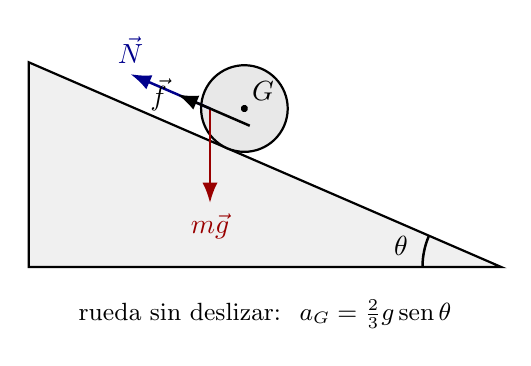
\begin{tikzpicture}[line width=0.9pt,>={Latex[length=2.6mm]}]
  % plano inclinado
  \coordinate (A) at (0,0); \coordinate (B) at (6,0); \coordinate (C) at (0,2.6);
  \draw[thick,fill=black!6] (A)--(B)--(C)--cycle;
  \draw ($(B)+(180:1.0)$) arc (180:157:1.0); \node at ($(B)+(168:1.3)$){$\theta$};
  % cilindro sobre la pendiente
  \begin{scope}[shift={($(C)!0.42!(B)$)},rotate=-23.4]
    \draw[thick,fill=black!9] (0,0.55) circle(0.55);
    \fill (0,0.55) circle(1.3pt) node[above right=-1pt]{$G$};
    % peso (vertical, no rotado): lo dibujo fuera del scope
  \end{scope}
  \coordinate (G) at ($(C)!0.42!(B)+(23.4:0)$);
  % recomputo G aprox
  \path ($(C)!0.42!(B)$) ++(113.4:0.55) coordinate (Gc);
  \draw[->,red!60!black] (Gc)--($(Gc)+(0,-1.2)$) node[below]{$m\vec g$};
  \draw[->,blue!55!black] (Gc)--($(Gc)+(156.6:1.1)$) node[above]{$\vec N$};
  \draw[->] (Gc)+(336.6:0.55) -- ($(Gc)+(336.6:0.55)+(156.6:1.0)$) node[left]{$\vec f$};
  \node at (3.0,-0.6){\small rueda sin deslizar: $\;a_G=\tfrac23 g\operatorname{sen}\theta$};
\end{tikzpicture}
\end{document}
